\appendix

\section{Triton erfcx approximation}\label{app:erfcx}

Because the GPU kernel compiler (Triton) lacks a native $\mathrm{erfcx}$ instruction, we implemented a piecewise approximation inside the fused kernel that combines a direct identity for $|z| \leq 3.5$ with a four-term asymptotic expansion for $|z| > 3.5$. For $z \geq 0$:
\begin{equation}
    \mathrm{erfcx}(z) \approx \begin{cases}
        e^{z^2}(1 - \mathrm{erf}(z)) & |z| \leq 3.5 \\[4pt]
        \displaystyle\frac{1}{z\sqrt{\pi}}\left(1 - \frac{1}{2z^2} + \frac{3}{4z^4} - \frac{15}{8z^6}\right) & |z| > 3.5
    \end{cases}
\end{equation}
For $z < 0$, we use the identity $\mathrm{erfcx}(z) = 2e^{z^2} - \mathrm{erfcx}(-z)$. For $|z| > 9$, the asymptotic form is applied unconditionally to prevent float32 overflow in the $e^{z^2}$ computation ($e^{81} \approx 5.3 \times 10^{35}$ is safe; $e^{88.7}$ exceeds float32 range). As $\tau \to 0$ after a renewal reset, $z \to -\infty$ and $\mathrm{erfcx}(z) \to \infty$, yielding $h_{\mathrm{LN}} \to 0$, which correctly reflects the biological reality that transition probability is zero immediately after entering a state.

We validate the approximation on a dense fp32-safe grid $z \in [-9, 30]$ (10{,}001 points); the upper negative bound is set by $\exp(z^2)$ overflowing single-precision at $|z| \gtrsim 9.4$, not by a limitation of the formula. The measured maximum relative error is $\sim$$4 \times 10^{-2}$ at $z \approx 3.5$, driven by catastrophic cancellation in the fp32 evaluation of $1 - \mathrm{erf}(z)$ precisely at the branch-switch, and drops to $\sim$$6 \times 10^{-3}$ away from the branch boundary. Because these errors enter the Bernoulli step as $1 - \exp(-\lambda_i \Delta t)$ with $\lambda_i \Delta t \lesssim \varepsilon = 0.03$, the induced bias in transition probability stays well below the structural-bias floor of synchronous tau-leaping itself ($\sim$6--7\%, Section~\ref{sec:validation}: $\sim$6\% peak-$I$ and $\sim$7\% final-$R$), so the approximation is comfortably within the tolerance of the stochastic integrator. A unit test (cited in the repository README) reproduces these bounds and guards against regressions. Random number generation uses Triton's native PRNG, seeded via a 64-bit host-managed step counter that increments by 1 per simulation step, preventing pattern repetition for over $2^{31}$ steps.

\section{Degree-heterogeneous graphs and auto-dispatch}
\label{app:degree_dispatch}

The 1-thread-per-node fused kernel introduced in Section~\ref{sec:fused_kernel} is optimal when the degree distribution is narrow, but degrades sharply on heavy-tailed topologies (scale-free, preferential-attachment, many real social networks). This appendix documents the two alternative CSR traversal kernels we provide, the auto-dispatch heuristic, and the measured gains, all consistent with Section~\ref{sec:csr_dispatch} and Table~\ref{tab:csr_dispatch}.

\subsection{Why the default kernel stalls on hubs}

In the 1-thread-per-node kernel, thread $i$ in a block of 128 threads iterates its own $D_i$ neighbors with a scalar \texttt{while} loop; all 128 threads in the block proceed to the per-node tail only when every thread's \texttt{while} has terminated. The block's wall-clock runtime is therefore $\bigO(\max_{i \in \text{block}} D_i)$. On a Barab\'{a}si--Albert graph with $N = 10^6$ and $m = 4$ the largest measured degree is $D_{\max} = 3{,}870$ ($D_{\max}/D_{\mathrm{avg}} = 484$), so any block containing even one hub stalls for 3{,}870 CSR iterations while 127 other threads have long since finished their degree-4 lists. Memory coalescing is also destroyed: the 128 threads are reading very different \texttt{col\_ind} offsets after the first few iterations. Measured fused-CG throughput collapses from $7.6$ Giga-NUPS on a regular degree-8 graph to $0.45$ Giga-NUPS on BA at the same $N$.

\subsection{Warp-per-node kernel}
\label{app:warp_kernel}

The first remediation cooperates within a warp: thread layout becomes $[\texttt{NODES\_PER\_BLOCK}, \texttt{LANES\_PER\_NODE}]$ with $\texttt{LANES\_PER\_NODE} = 32$, one warp per node. Each warp iterates the node's neighbor list in chunks of 32 edges, using a 2D register tile for partial pressures; at the end a \texttt{tl.sum} along the lane axis collapses the tile to a per-node scalar. Hub traversal now takes $\lceil D_{\max} / 32 \rceil$ warp-parallel iterations rather than $D_{\max}$ serial ones.

The per-node tail (hazard evaluation, Bernoulli sampling, transition, next-infectivity write) re-uses the 1D code path of the baseline kernel on a \texttt{NODES\_PER\_BLOCK}-element tensor; only those few lanes produce meaningful writes, so a moderate amount of block-wide ALU/memory bandwidth is wasted there. The tradeoff is favorable for hub-containing blocks but loses on uniform-degree graphs because the CSR coalescing that the baseline enjoys is given up (most lanes do useless work in any given chunk when $D_i \ll 32$).

We verified bit-identical per-step parity of the warp kernel against the baseline on both a regular degree-8 graph and a BA graph at $N = 10^4$ over 50 steps, using the deterministic \texttt{tl.rand(seed + step\_id, node\_id)} RNG pattern shared across kernels. Zero mismatches were observed in \texttt{state}, \texttt{age}, \texttt{infectivity}, or \texttt{rates} at any step.

\subsection{Edge-partitioned merge-based kernel}
\label{app:merge_kernel}

The second remediation is a merge-path load-balancer along the lines of \citet{merrill2016merge}: each program processes a fixed chunk of $\texttt{EDGES\_PER\_BLOCK}$ contiguous edges (not nodes), independent of which nodes those edges belong to. Each thread in the program handles one edge and performs:
\begin{enumerate}
\item Load $(\texttt{col\_ind}[e], \texttt{weights}[e], \texttt{infectivity}[\texttt{col\_ind}[e]])$.
\item Recover the source node id $n$ such that $\texttt{row\_ptr}[n] \leq e < \texttt{row\_ptr}[n+1]$ via a fully unrolled binary search of depth $\lceil \log_2(N + 2)\rceil$ over \texttt{row\_ptr}.
\item Atomic-add the weighted contribution $\texttt{infectivity}[\texttt{col\_ind}[e]] \cdot \texttt{weights}[e]$ to a pressure scratch buffer at index $n$.
\end{enumerate}
A second lightweight kernel (\texttt{\_flash\_renewal\_tail\_kernel}) then reads the pressure buffer and runs the unchanged per-node tail: hazard, Bernoulli, transition, next-infectivity write. Because the two kernels share the same RNG pattern as the single-kernel variants, they produce statistically identical trajectories.

Load balance across blocks is now perfect regardless of degree skew --- every block does exactly $\texttt{EDGES\_PER\_BLOCK}$ worth of work. The price is (i) one atomic add per edge (contention dominated by hubs, but still much faster than the baseline's serial hub traversal), (ii) a scratch buffer read/write of $4N$ bytes, and (iii) one extra kernel launch per step. The scheme pays off when degree skew is large enough that the baseline's idle-warp waste exceeds these fixed costs.

\subsection{Auto-dispatch}

At engine construction \flashspread{} inspects \texttt{row\_ptr} once, computes $\rho = D_{\max}/D_{\mathrm{avg}}$, and selects:
\begin{equation}
\text{strategy}(\rho) = \begin{cases}
\texttt{thread} & \rho < 4, \\
\texttt{warp}   & 4 \leq \rho < 50, \\
\texttt{merge}  & \rho \geq 50.
\end{cases}
\end{equation}
The thresholds are calibrated from the sweep in Table~\ref{tab:degree_dispatch_sweep}. The user can override via an explicit \texttt{csr\_strategy} argument. The dispatch cost is one pass over \texttt{row\_ptr} at construction ($\bigO(N)$, amortized trivially over every subsequent step).

\subsection{Parity and throughput}

\textbf{Parity.} We ran the three strategies on $N = 10^4$ regular-degree-8 and BA-$m{=}4$ graphs for 50 tau-leaping steps with a deterministic seed. The \texttt{thread} and \texttt{warp} kernels produced bit-identical per-node outputs (\texttt{state}, \texttt{age}, \texttt{infectivity}, \texttt{rates}) at every step. The \texttt{merge} kernel uses non-deterministic atomic-add ordering and therefore can differ by fp rounding at the LSBs of the pressure buffer; over our 50-step window on both graphs the SEIR population counts matched bit-exactly (zero delta in all four bins) because no Bernoulli draw landed within fp ULP of its threshold.

\textbf{Throughput.} Table~\ref{tab:degree_dispatch_sweep} shows the full tunable sweep on both graphs at $N = 10^6$ (Fused CG $b = 50$, A100, same experimental setup as Section~\ref{sec:experiments}).

\begin{table}[H]
\caption{Full CSR-strategy throughput sweep on ER and BA at $N = 10^6$, Fused CG, $b = 50$, A100. NPB = \texttt{NODES\_PER\_BLOCK} (warp); EPB = \texttt{EDGES\_PER\_BLOCK} (merge). Bold entries denote the strategy auto-dispatch picks for that graph.}
\label{tab:degree_dispatch_sweep}
\centering
\begin{tabular*}{\linewidth}{@{}llcc@{}}
\toprule
\textbf{Strategy}             & \textbf{Tunable}   & \textbf{Regular $d=8$} & \textbf{BA $m=4$} \\
                              &                    & G-NUPS               & G-NUPS \\
\midrule
\texttt{thread}               & ---                & \textbf{7.88}        & 0.45 \\
\midrule
\texttt{warp}                 & NPB = 2            & 0.86                 & 0.75 \\
\texttt{warp}                 & NPB = 4            & 1.37                 & 1.16 \\
\texttt{warp}                 & NPB = 8            & 1.70                 & 1.30 \\
\midrule
\texttt{merge}                & EPB = 1{,}024      & 3.92                 & \textbf{2.00} \\
\texttt{merge}                & EPB = 2{,}048      & 3.44                 & 1.78 \\
\texttt{merge}                & EPB = 4{,}096      & 3.35                 & 1.86 \\
\texttt{merge}                & EPB = 8{,}192      & 1.41                 & 0.84 \\
\midrule
\textbf{Auto-dispatch gain}    & vs.\ \texttt{thread} & $1.00\times$       & $\mathbf{4.48\times}$ \\
\bottomrule
\end{tabular*}
\end{table}

Key observations:
\begin{itemize}
\item On the regular graph ($\rho = 2$), every alternative strategy is strictly worse than \texttt{thread}; auto-dispatch correctly chooses \texttt{thread}, so the user pays nothing for having the machinery available.
\item On BA ($\rho = 484$), \texttt{merge} outperforms \texttt{warp} by $\sim$50\% at the best tuning (EPB = 1{,}024 wins over NPB = 8), and both outperform \texttt{thread}.
\item The \texttt{warp} strategy is not currently a winner in the auto-dispatch decision (\texttt{merge} strictly dominates it for $\rho \geq 50$ in our sweep), but we retain it for two reasons: its per-block register-tile accumulation is atomic-free and deterministic bit-to-bit (useful for reproducibility-critical users), and its optimal regime $4 \leq \rho < 50$ covers medium-heterogeneity graphs on which the \texttt{merge} scheme's atomic contention would be unnecessary overhead.
\item EPB = 1{,}024 is the sweet spot on both graphs. Smaller EPB increases launch overhead; EPB = 8{,}192 concentrates too many atomic targets per block and the scheduler can't hide the contention behind other work.
\end{itemize}

Combining the contributions in Section~\ref{sec:renewal_engine} and Section~\ref{sec:csr_dispatch}, the end-to-end speedup chain on BA at $N = 10^6$ is: exact CPU Phantom Process \citep{vajdi2020stochastic} $\approx$ 70 transitions/sec; CPU tau-leaping $\approx$ 37 M-NUPS ($5 \times 10^5\times$ from algorithmic relaxation); 1-thread-per-node fused CG on BA $= 0.45$ G-NUPS ($12\times$ hardware from the naive GPU); auto-dispatched merge-based fused CG on BA $= 2.0$ G-NUPS ($4.5\times$ from degree-aware dispatch). Every factor is strict-hardware (no algorithmic relaxation past the tau-leaping baseline), and the entire chain reproduces end-to-end from the repository; the README names the harness that regenerates these numbers.

\section{Tau-leaping fidelity and compute budgeting}
\label{app:fidelity}

The fused Bernoulli tau-leaping of Algorithm~\ref{alg:fused} introduces two distinct sources of error relative to the exact continuous-time stochastic process on the network: a \emph{discretization} error from finite $\Delta t$ that vanishes as $\varepsilon \to 0$, and a \emph{structural} error from synchronous per-step updates that does not. This appendix quantifies both on the standard SEIR benchmark ($N = 10^3$, ER $d = 8$, log-normal $E\to I$ and $I\to R$, $\beta = 2/d$, 100 runs), maps the fidelity--compute Pareto frontier, and gives a practical rule for choosing $\varepsilon$ under a given compute budget.

\subsection{Two sources of error}

\paragraph{Discretization.} The per-node Bernoulli step probability $p_i = 1 - \exp(-\lambda_i \Delta t)$ is exact only when $\lambda_i$ is constant on $[t, t + \Delta t)$. For non-Markovian hazards $h(\tau)$ the rate varies smoothly within a step; for Markovian rates it changes discretely whenever a neighbor transitions. Both effects contribute an $\bigO(\varepsilon)$ bias in the expected transition count per step. Reducing $\varepsilon$ tightens the integration at the cost of more steps per trajectory, up to the point where per-step cost becomes negligible and only the structural term remains.

\paragraph{Structural.} Within a single tau-leap, all nodes sample Bernoulli trials against their \emph{begin-of-step} rate; transitions are then applied simultaneously. This omits the (non-negligible) event that node $u$ transitions mid-step and alters node $v$'s rate before $v$ samples. Exact Gillespie captures this by ordering events one at a time; tau-leaping does not. The structural bias is therefore a property of synchronous updates on the network and is independent of $\varepsilon$: it vanishes only in the thermodynamic / mean-field limit, or when the per-node rate is so small that at most one transition per Bernoulli window is a valid approximation.

\subsection{Fidelity metrics}

We report four metrics of the ensemble-mean trajectory $(\hat S, \hat E, \hat I, \hat R)(t)$ against the exact Gillespie reference $(S, E, I, R)(t)$:
\begin{itemize}
\item Trajectory $L_\infty$: $\max_{t, s} |\hat y_s(t) - y_s(t)|$ over time and compartment.
\item Trajectory $L_2$: $\sqrt{\overline{(\hat y_s(t) - y_s(t))^2}}$ over the 501-point sample grid.
\item Peak-infection error: $|\max_t \hat I(t) - \max_t I(t)|$.
\item Final-attack-rate error: $|\hat R(T) - R(T)|$ at $T = 50$.
\end{itemize}
For the appendix plots we additionally report a \emph{self-consistency} error against our finest discretization ($\varepsilon = 0.005$, 100 runs) as a proxy for the discretization component alone, isolated from the structural bias.

\subsection{Empirical convergence}

Figure~\ref{fig:fidelity_traj} overlays ensemble-mean trajectories of four $\varepsilon$ values. Qualitatively, $\varepsilon = 0.1$ already tracks the $\varepsilon = 0.005$ reference across all four compartments; reductions below $\varepsilon \approx 0.03$ change the curves only imperceptibly at plot resolution.

\begin{figure}[H]
\centering
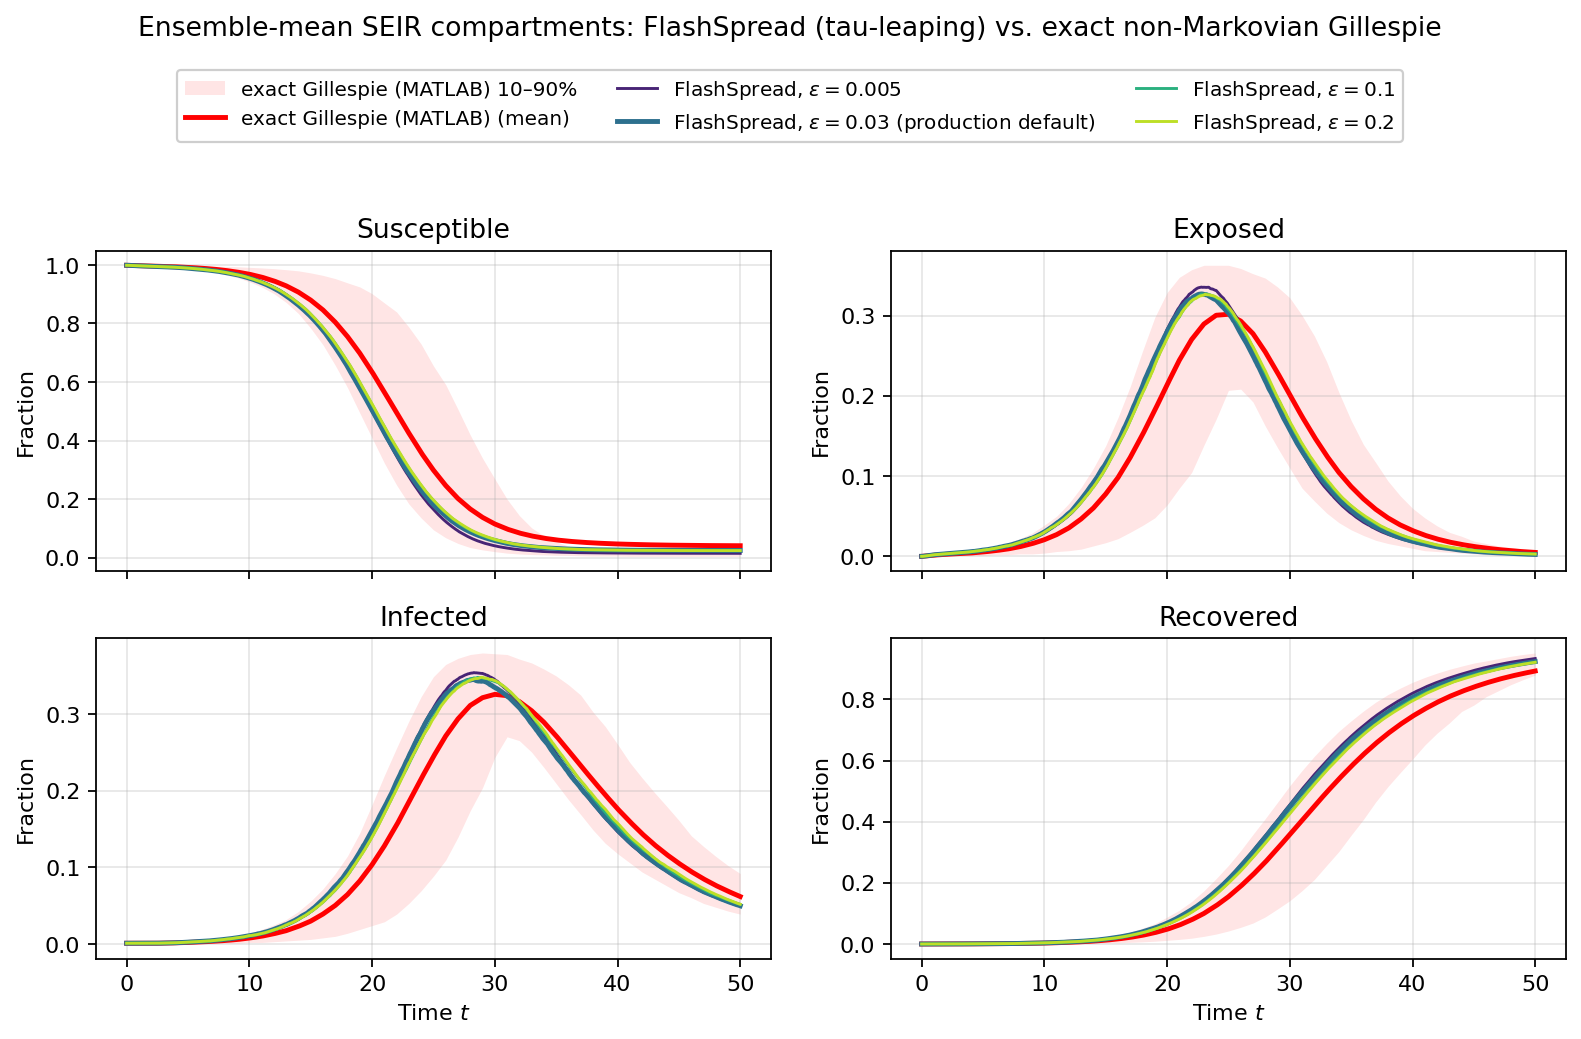
\includegraphics[width=0.98\columnwidth]{figures/fig_fidelity_traj.png}
\caption{Ensemble-mean SEIR trajectories overlaid on the exact non-Markovian Gillespie reference (red solid, with 10--90\% Monte Carlo quantile band), plus four tau-leaping tolerances, on the validation benchmark (Erd\H{o}s--R\'{e}nyi graph with $N = 10^3$ nodes and average degree $d = 8$; $\beta = 2/d = 0.25$; log-normal $E{\to}I$ and $I{\to}R$ with the parameters of Section~\ref{sec:experiments}; 100 independent Monte Carlo trajectories per curve). The exact reference is the companion MATLAB implementation of the non-Markovian Gillespie algorithm \citep{boguna2014simulating}. The $\varepsilon = 0.005$ tau-leaping curve (black) is the practical discretization limit; coarser $\varepsilon$ deviates smoothly but tracks the exact curve tightly. The residual offset between every tau-leaping curve and the exact reference is the structural bias of synchronous Bernoulli updates on a network, independent of $\varepsilon$.}
\label{fig:fidelity_traj}
\end{figure}

Figure~\ref{fig:fidelity_err_eps} shows the quantitative picture on log-log axes, with per-run error bars from a 1{,}000-resample bootstrap over the 100 Monte Carlo trajectories. The peak-$I$ and final-$R$ errors \emph{against exact Gillespie} (solid markers) are statistically indistinguishable across two decades of $\varepsilon$: the 95\% CI envelopes of adjacent $\varepsilon$ values overlap, so the apparent non-monotonicity in the point estimates is ensemble-sampling noise rather than a true convergence pattern. To convert this visual claim into a quantitative one, we fit $\log_{10} \text{err} = \alpha \log_{10} \varepsilon + c$ across the full $\varepsilon \in [0.005, 0.2]$ sweep and bootstrap the slope $\alpha$ over 5{,}000 resamples: the fitted slopes are $\alpha_{\text{peak-}I} = +0.024$ with 95\% CI $[-0.026,\, +0.053]$ and $\alpha_{\text{final-}R} = +0.031$ with 95\% CI $[-0.106,\, +0.116]$. Both intervals contain zero, so the hypothesis of no log-linear decrease of the exact-reference error with $\varepsilon$ is not rejected at the $0.05$ level; if anything, the point estimates are slightly positive, consistent with the structural bias being an $\varepsilon$-independent floor rather than a vanishing error term. In contrast, the self-consistency $L_\infty$ and $L_2$ metrics (dashed, vs the $\varepsilon = 0.005$ ensemble) decrease monotonically with $\varepsilon$: this is the pure discretization component. The separation between the two sets of curves is the \emph{structural bias floor}.

\begin{figure}[H]
\centering
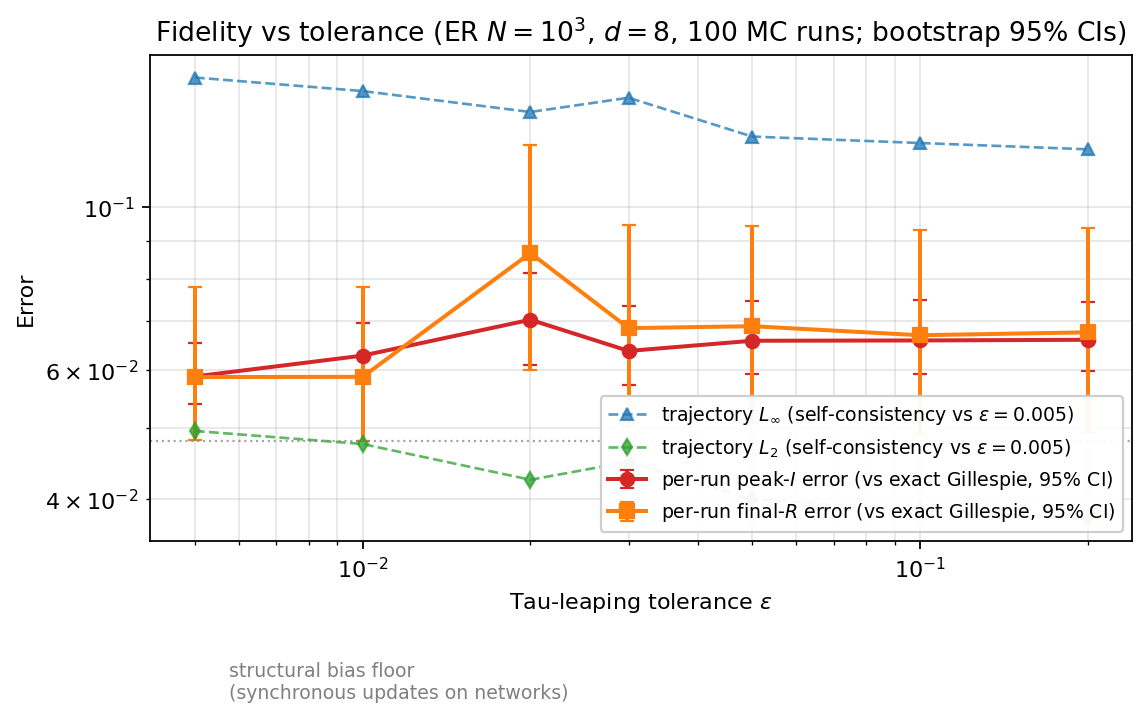
\includegraphics[width=0.98\columnwidth]{figures/fig_fidelity_err_vs_eps.png}
\caption{Error decomposition for Bernoulli tau-leaping, with bootstrap 95\% confidence intervals over the 100-run ensemble. Solid markers (with error bars) are per-run absolute errors against the exact non-Markovian Gillespie reference produced by the companion MATLAB simulator. Dashed markers are self-consistency trajectory-level errors against the finest $\varepsilon = 0.005$ tau-leaping ensemble. The solid curves' CIs overlap and sit at the structural bias floor (dotted grey), showing that within ensemble noise the peak-$I$ and final-$R$ errors do not detectably decrease below $\sim$6\% as $\varepsilon \to 0$ across the sweep; the dashed curves continue decreasing as pure discretization error vanishes. Below $\varepsilon \approx 0.1$ the structural term dominates and further reductions in $\varepsilon$ buy no detectable fidelity improvement on this benchmark.}
\label{fig:fidelity_err_eps}
\end{figure}

\subsection{Robustness across topologies and sizes}
\label{app:fidelity_multi}

The single-graph result above could in principle be an artefact of the particular sparse ER topology or of the $N = 10^3$ scale. To rule that out, we repeat the sweep over three qualitatively different graph families --- sparse Erd\H{o}s--R\'{e}nyi ($d=8$), scale-free Barab\'{a}si--Albert ($m=4$, average degree $\approx 8$, $D_{\max}$ growing with $N$), and deterministic fixed-degree ($d=8$, homogeneous) --- and three network sizes ($N \in \{10^3, 10^4, 10^5\}$). For each $(G, N, \varepsilon)$ cell we average 20 Monte Carlo trajectories. To keep the ensemble-mean informative, initial seeding is $\max(10,\; 0.01 N)$ Exposed nodes at $t = 0$, well above the stochastic-fadeout threshold on all three topologies; this lets us focus the comparison on the bulk epidemic dynamics rather than the early extinction-prone phase.

Figure~\ref{fig:fidelity_multi} shows the resulting $I(t)/N$ curves. Four properties are robust across the grid:
\begin{itemize}
\item At every $(G, N)$ the $\varepsilon = 0.1$ trajectory lies visually on top of the $\varepsilon = 0.005$ reference; the small gap between them is the discretization component and is insensitive to topology or scale.
\item Epidemic \emph{shape} depends on topology. ER and fixed-degree give similar symmetric peaks near $t \approx 25$; BA's heavy-tailed degree distribution produces an earlier takeoff and a wider peak, because the few high-degree hubs reach saturation faster than the network average.
\item Epidemic \emph{size} depends on $N$. On ER the peak fraction is near-stationary around $0.37$; on BA it drifts slightly with $N$ because the hub fraction changes. The tau-leaping--to--reference agreement holds at every $N$ individually.
\item The agreement-across-$\varepsilon$ story is preserved: the curve at $\varepsilon = 0.1$ tracks the reference to within plot resolution on every panel, which is the main fidelity claim of the appendix, tested against topology and scale simultaneously.
\end{itemize}

\begin{figure}[H]
\centering
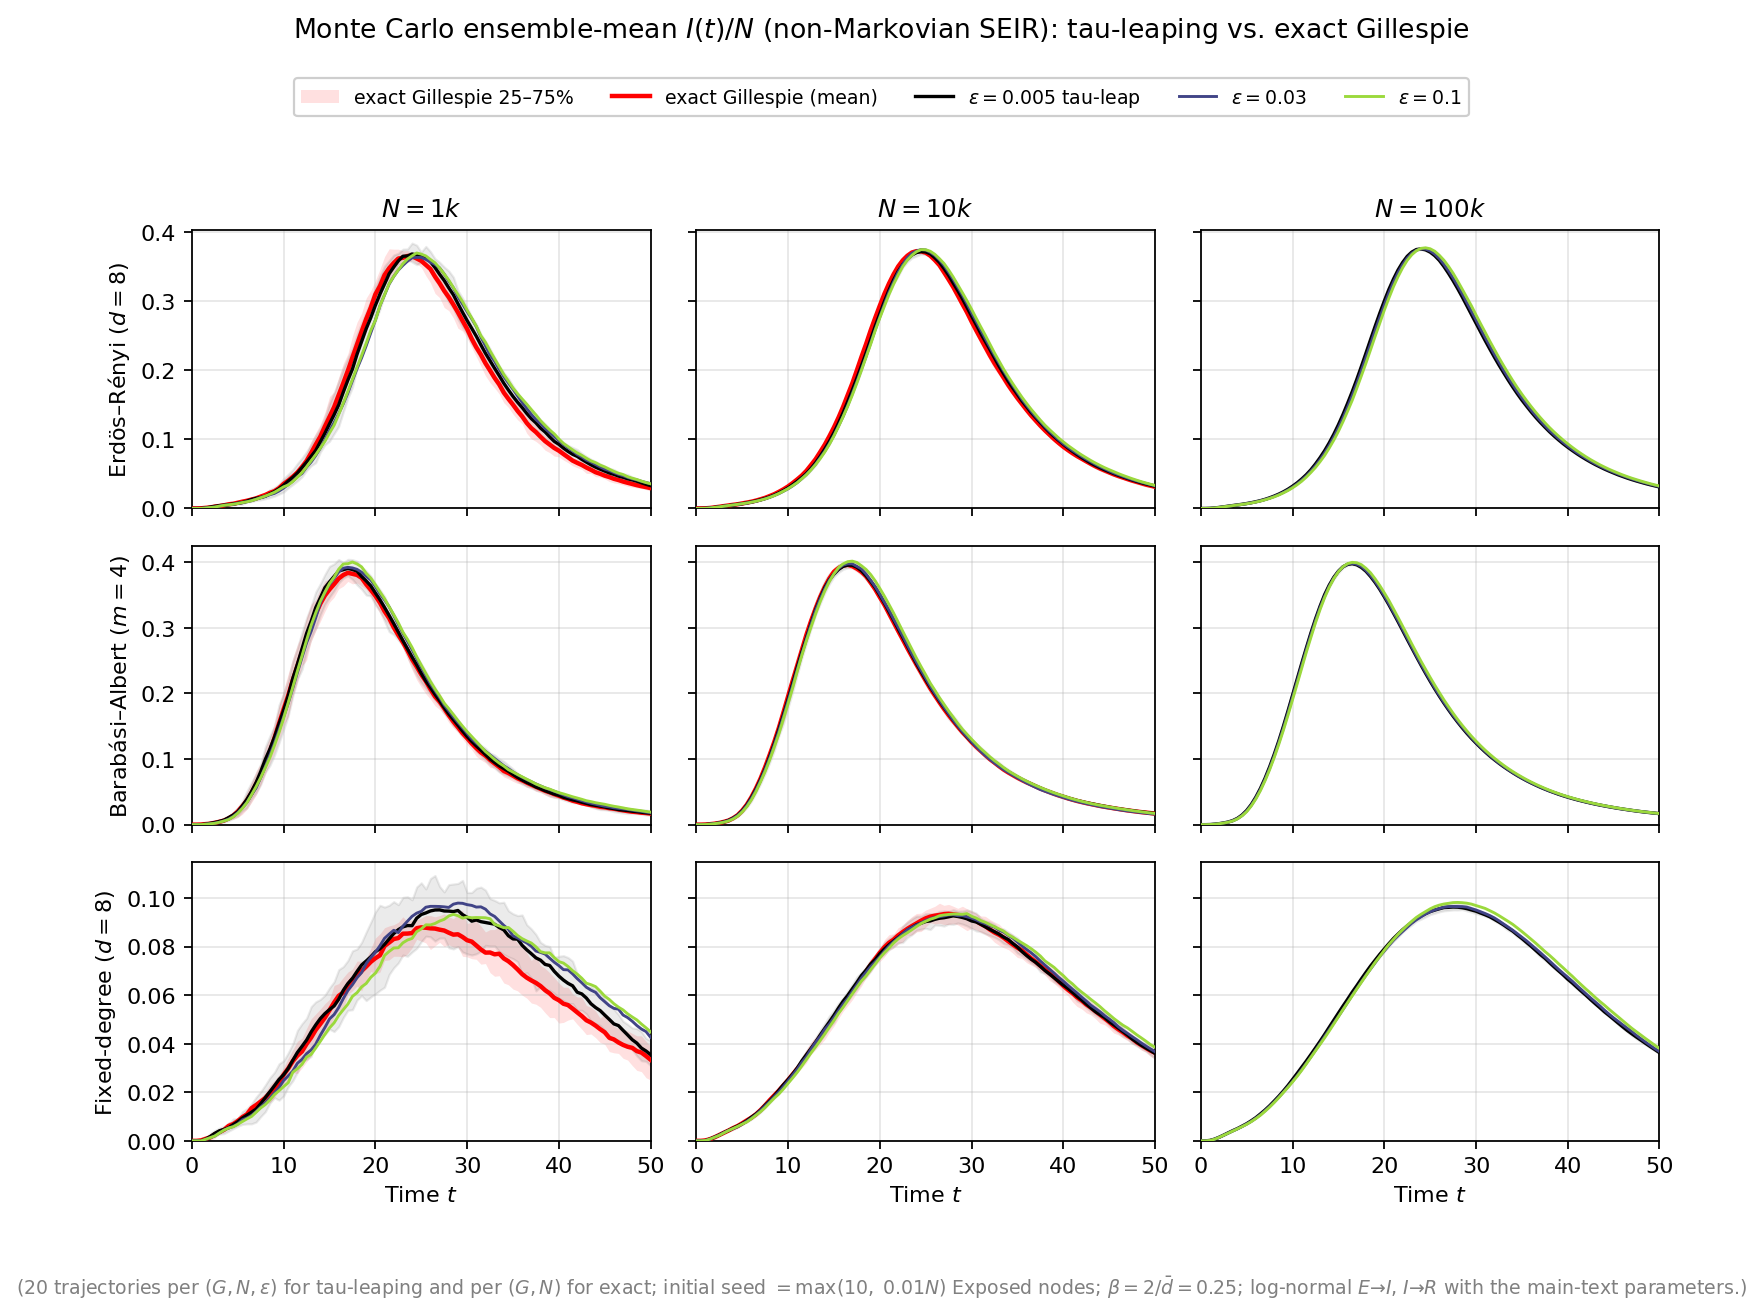
\includegraphics[width=0.96\textwidth]{figures/fig_fidelity_multi.png}
\caption{Monte Carlo ensemble-mean $I(t)/N$ for the non-Markovian SEIR model (log-normal $E{\to}I$ and $I{\to}R$) across three graph topologies (rows) and three sizes (columns). Each panel overlays an exact non-Markovian Gillespie reference (red, with 25--75\% inter-quartile band shaded; implemented via our companion CPU simulator, cited in the repository README) and tau-leaping at $\varepsilon \in \{0.005, 0.03, 0.1\}$ (the $\varepsilon = 0.005$ curve is the discretization-limit reference in black). Exact reference curves are provided for $N \in \{10^3,\,10^4\}$; $N = 10^5$ is beyond the CPU-Gillespie budget for 20 trials but is covered by tau-leaping alone. Every epidemic takes off (initial seed of $\max(10,\; 0.01 N)$ Exposed nodes) and the tau-leaping curves are indistinguishable from the exact Gillespie curve at plot resolution across all covered cells, demonstrating that the fidelity story established at $N = 10^3$ on ER transfers directly to scale-free and homogeneous topologies and to sizes up to $10^5$.}
\label{fig:fidelity_multi}
\end{figure}

\subsection{Compute--fidelity Pareto}

Figure~\ref{fig:fidelity_pareto} plots mean wall-clock per trajectory against $\max(\text{err peak-}I,\; \text{err final-}R)$ versus exact, with bootstrap 95\% CIs on both axes. Within those CIs the error metric is statistically flat across $\varepsilon \in [0.005, 0.2]$ while wall-clock scales as $\sim 1/\varepsilon$ below the $\tau_{\max}$-clamp region. Any point strictly above the fastest one (top-right of the overlap band) pays compute for no statistically significant fidelity gain, and in particular $\varepsilon = 0.005$ is almost always wasteful on this benchmark.

\begin{figure}[H]
\centering
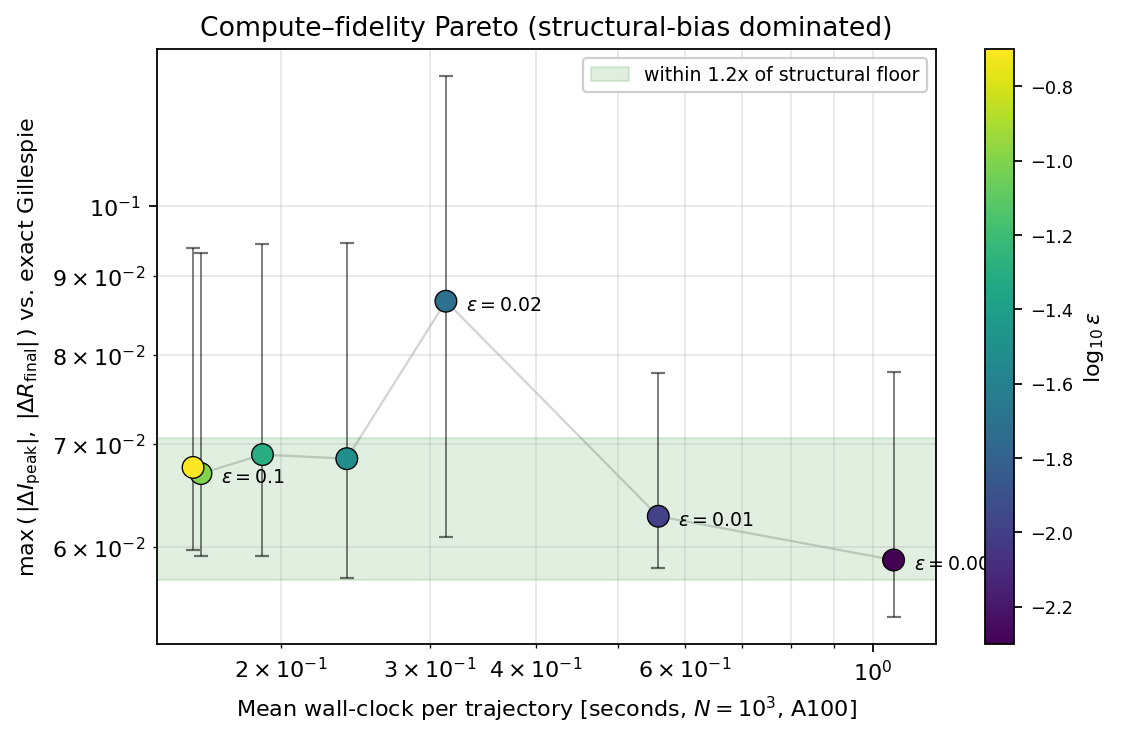
\includegraphics[width=0.98\columnwidth]{figures/fig_fidelity_pareto.png}
\caption{Wall-clock--fidelity Pareto. Each point is one $\varepsilon$ value (color: $\log_{10}\varepsilon$, labelled). The vertical axis is $\max(|\Delta I_{\mathrm{peak}}|,\,|\Delta R_{\mathrm{final}}|)$ --- the larger of the two per-run absolute errors against the exact Gillespie reference --- chosen so that no metric can hide a worse metric. Error bars on both axes are 95\% bootstrap CIs (1{,}000 resamples over the 100-run ensemble): horizontal bars for wall-clock, vertical bars for the fidelity metric. The vertical CIs overlap across two decades of $\varepsilon$ while wall-clock spans a factor of seven: above the fast-end cluster, additional compute does not translate into statistically detectable fidelity gains.}
\label{fig:fidelity_pareto}
\end{figure}

\subsection{Tuning rules}

From the Pareto analysis we extract a simple rule of thumb, summarised in Table~\ref{tab:fidelity_budget}. The numbers are calibrated to this benchmark; the underlying logic --- choose the largest $\varepsilon$ that keeps you in the flat portion of the curve --- transfers to other topologies and parameter regimes.

\begin{table}[H]
\caption{Recommended $\varepsilon$ by compute budget and application. All timings are for $N = 10^3$ single-trajectory wall-clock on an A100, from the fidelity sweep plotted in Figures~\ref{fig:fidelity_err_eps}--\ref{fig:fidelity_pareto}. The err peak-$I$ column is the per-run mean against the exact non-Markovian Gillespie reference produced by the companion MATLAB simulator on the same graph and parameters, with the 95\% bootstrap CI in brackets (1{,}000 resamples over 100 Monte Carlo runs). The CI envelopes overlap between adjacent rows: within finite-ensemble noise the err peak-$I$ is flat across two decades of $\varepsilon$ while wall-clock varies by a factor of $\sim$7. Reducing $\varepsilon$ below $\sim$0.03 buys compute, not fidelity, on this benchmark, which is why the main text uses $\varepsilon = 0.03$ as the default; $\varepsilon = 0.1$ is a viable aggressive-throughput alternative when structural bias is known to dominate and per-trajectory fidelity is not the scoring metric (e.g., bulk RL training). Rows are ordered from fastest to slowest.}
\label{tab:fidelity_budget}
\centering
\begin{tabular*}{\linewidth}{@{}lccc@{}}
\toprule
\textbf{Use case}                              & $\varepsilon$ & \textbf{err peak-$I$ (95\% CI)} & \textbf{wall-clock (95\% CI)} \\
\midrule
Aggressive throughput (RL training, ensembles) & 0.2  & 6.60\% [5.98, 7.42]  & 0.157~s [0.157, 0.158] \\
RL training / bulk ensemble sampling           & 0.1  & 6.59\% [5.92, 7.49]  & 0.161~s [0.160, 0.161] \\
Default (forecasts, policy evaluation)         & 0.03 & 6.37\% [5.73, 7.33]  & 0.239~s [0.236, 0.241] \\
Publication-quality validation                 & 0.01 & 6.28\% [5.82, 6.97]  & 0.558~s [0.547, 0.565] \\
Over-resolved (almost always wasteful)         & 0.005& 5.88\% [5.40, 6.53]  & 1.058~s [1.033, 1.079] \\
\bottomrule
\end{tabular*}
\end{table}

\paragraph{When the rule of thumb breaks.}
The recommendation $\varepsilon = 0.1$ is tied to the observation that structural bias dominates here. Two regimes where the discretization term dominates instead, and where $\varepsilon$ should be reduced towards $0.01$:
\begin{itemize}
\item \emph{Near-mean-field / large-$N$ regimes}, where the structural bias vanishes (Starnini et al., and the correspondence literature discussed in Section~\ref{sec:related}). In these regimes discretization is the only error source and $\varepsilon$ should be chosen directly from the $\bigO(\varepsilon)$ Bernoulli integration bound.
\item \emph{Highly non-Markovian dynamics with sharply peaked hazards}, where the per-step rate change is large (e.g., log-normal shedding profiles with small $\sigma$). Here the begin-of-step rate is a poor approximation of the integrated rate, and a smaller $\varepsilon$ is warranted.
\end{itemize}
A single short run at $\varepsilon \in \{0.1, 0.03\}$ on any new workload is typically enough to tell which regime one is in: if the two agree to within 1\% on the target metric, keep $\varepsilon = 0.1$; otherwise step down to $\varepsilon = 0.03$ and re-check.

The sweep in this appendix is reproducible from the repository; the README lists the data-generation and plotting scripts.

\subsection{Markovian SIS / SIR validation: exact protocol and reproducibility pointer}
\label{app:sis_sir}

Section~\ref{sec:markov_validation} presents the headline result; the IQR-band agreement and regime separation between SIS and SIR are discussed there. This appendix exists only to document the protocol with enough detail to reproduce the run from the public repository, without repeating the result prose in the main text.

\textbf{Parameters.} Erd\H{o}s--R\'{e}nyi graph with $N = 10^3$ nodes and average degree $d = 8$, $\beta = 0.25$, initial seed of 10 infected nodes, recovery rate $0.15$ (either $\delta$ for SIS or $\gamma$ for SIR), 100 independent Monte Carlo runs.

\textbf{Implementations.} The exact reference is a standard Doob--Gillespie direct-method simulator maintained incrementally; the FlashSpread side uses the public \textsc{MarkovianEngine} with its default adaptive tau-leaping sampler at \texttt{max\_prob = 0.1} and \texttt{theta = 0.01}. No parameter tuning beyond those defaults was performed.

\textbf{Reproducibility.} Both simulators, their SLURM wrappers, and the post-processing that produced Figure~\ref{fig:sis_sir_validation} are listed in the ``Reproducing the Paper'' section of the repository README against the \texttt{jocs-submission} tag.

\section{Data layout, FlashNeighbor, and the GPU memory flow}
\label{app:data_flow}

Section~\ref{sec:engines} described the FlashNeighbor kernel at a high level: one thread per node, gather-based CSR traversal, no atomics, a single write-back per thread. This appendix fills in the concrete data layout, the per-thread execution pattern, and the corresponding traffic through the GPU memory hierarchy. These details drive the asymptotic figures quoted in Section~\ref{sec:fused_kernel} ($\sim$64$N$ bytes unfused $\to$ $\sim$20$N$ bytes fused) and the $\bigO((N{+}E)/P)$ per-step complexity claimed throughout the paper.

\subsection{Compressed sparse row (CSR) representation}
\label{app:csr}

\flashspread{} stores the contact network in Compressed Sparse Row (CSR) form, \emph{indexed by incoming edges}, with a mirrored outgoing CSR maintained only for the Markovian Inertial-Mode sparse update path (Section~\ref{sec:markov_engine}). Figure~\ref{fig:csr_layout} traces one node through the three arrays.

\begin{figure}[H]
\centering
\includestandalone[width=0.98\columnwidth]{figures/fig-csr-layout}
\caption{CSR layout used throughout \flashspread{}. Left: a small undirected contact graph; node 2 (red) is the focus. Right: the three CSR arrays. \texttt{row\_ptr[i..i+1)} delimits node $i$'s neighbor slice in \texttt{col\_ind} and \texttt{weights}. Reading node 2's neighbors therefore costs two coalesced scalar loads (pointer endpoints) plus a contiguous burst of $D_2$ int/float pairs. Incoming and outgoing CSRs are stored separately: the incoming copy drives both engines' FlashNeighbor reads; the outgoing copy drives Inertial-Mode sparse atomic propagation when a single node transitions.}
\label{fig:csr_layout}
\end{figure}

The layout has three properties that the kernel design exploits:
\begin{itemize}
\item \emph{Contiguity.} A node's neighbors occupy a contiguous slice of \texttt{col\_ind} and \texttt{weights}. A warp of threads processing one node therefore issues a coalesced burst load; a block of threads processing one-node-per-thread produces $B$ scattered bursts, where $B$ is the thread-block size.
\item \emph{Cacheability.} On an A100, L2 is $\sim$40~MB, shared among all SMs. A CSR for $N = 10^6$ and $d = 8$ (\texttt{col\_ind} $+$ \texttt{weights}) totals $64$~MB and no longer fits; the ``L2 cache cliff'' at $N = 10^7$ (Figure~\ref{fig:throughput_renewal}) is this effect. Auto-dispatch does not change the data layout but changes the \emph{access order}, which is what determines whether the L2 miss pattern stays tractable on scale-free graphs (Appendix~\ref{app:degree_dispatch}).
\item \emph{Memory footprint} is $4(N{+}1)$ bytes (\texttt{row\_ptr}, int32) $+\,4E$ (\texttt{col\_ind}, int32) $+\,4E$ (\texttt{weights}, fp32) $=\,8E + 4(N{+}1)$ bytes for the incoming copy, doubled when the outgoing copy is present. At $N = 10^6$, $d = 8$ (directed edge count $E = 8N = 8 \times 10^6$), this is $8 \cdot 8 \times 10^6 + 4 \cdot (10^6{+}1) \approx 68$~MB per copy (dominated by the $8E$ edge payload; we abbreviate as ``$\sim$64~MB'' elsewhere in the text when quoting the $8E$ edge term alone). At $N = 10^7$ the same formula gives $\sim$680~MB per copy, which is where the L2 cache cliff in Figure~\ref{fig:throughput_renewal} sets in. The $N \lesssim 10^8$ single-GPU ceiling quoted in the paper follows directly from doubling this footprint plus $\bigO(N)$ per-node state ($4N + 4N + 4N + 4N$ bytes for \texttt{state}, \texttt{age}, \texttt{infectivity}, \texttt{rates}) and fitting in the A100's 40--80~GB of HBM.
\end{itemize}

\subsection{FlashNeighbor: per-thread execution inside one fused launch}
\label{app:flashneighbor}

The kernel maps one GPU thread to one target node $i$, with no shared memory and no atomics. Figure~\ref{fig:flashneighbor} shows the data flow for a single warp.

\begin{figure}[H]
\centering
\includestandalone[width=0.96\textwidth]{figures/fig-flashneighbor}
\caption{FlashNeighbor kernel, per-thread view. Each thread owns a unique target node $i$ and accumulates its influence $p_i$ in a private register. The loop body reads \texttt{row\_ptr[i..i+1)} once (coalesced), then iterates the neighbor slice: each iteration issues one indirect gather into \texttt{col\_ind}, one coalesced load of \texttt{weights}, and one indirect gather into the \texttt{infectivity} buffer (the L2 path is the only place these dashed loads land because they are node-indirect). The accumulation $p_i \mathrel{+}= w_{ij}\,\iota_{c_{ij}}$ lives entirely in the thread's register file; the kernel never touches shared memory. At the end of the loop the thread performs exactly \emph{one} fp32 store back to HBM for its node. No atomic operations are required because each target $i$ is uniquely owned.}
\label{fig:flashneighbor}
\end{figure}

Three implementation details make this efficient:
\begin{enumerate}
\item \emph{Write-once output.} The per-thread pressure $p_i$ is a register-resident fp32 accumulator during the whole loop; it materializes in HBM only once, at kernel end. In the unfused pipeline this single register value became a full $\bigO(N)$ intermediate tensor between two kernels.
\item \emph{Indirect gather cost is paid once per edge.} Each edge $(i,j)$ contributes three memory transactions on the read side: \texttt{col\_ind[e]} (coalesced), \texttt{weights[e]} (coalesced), and \texttt{infectivity[col\_ind[e]]} (gather, potentially L2-resident if the neighbor $j$ was recently touched). The gather is the bandwidth-bound operation; the coalesced loads ride in the shadow of its latency.
\item \emph{Block-level sparsity} (Section~\ref{sec:fused_kernel}) is applied \emph{after} the pressure accumulation, as part of the hazard-evaluation stage in the same launch. The reduction $\texttt{any\_e}$, $\texttt{any\_i}$ is a warp shuffle, essentially free, so the kernel never materialises a mask tensor.
\end{enumerate}

In Appendix~\ref{app:degree_dispatch} we replace step 1's ``one thread per node'' by either ``one warp per node'' (for $\rho \geq 4$) or ``one thread per edge'' with binary-search node attribution (for $\rho \geq 50$). The \emph{data layout} is identical in all three cases; only the thread-to-work mapping changes.

\subsection{Flow through the GPU memory hierarchy}
\label{app:memory_flow}

The reason kernel fusion matters on this workload is not FLOP count but HBM traffic. Figure~\ref{fig:memory_flow} contrasts the legacy unfused pipeline (five separate kernels, each materialising an $\bigO(N)$ intermediate tensor to HBM) with the fused kernel (all intermediates stay in SM registers for the lifetime of one per-node pipeline).

\begin{figure}[H]
\centering
\includestandalone[width=0.96\textwidth]{figures/fig-memory-flow}
\caption{GPU memory-hierarchy flow, before and after fusion. \textbf{(a)} The legacy PyTorch/Triton pipeline launches five kernels per step; each kernel reads from HBM and writes its $\bigO(N)$ intermediate (infectivity, pressure, rates, event probabilities, event mask) back to HBM before the next kernel starts. Total traffic is $\sim$64$N$ bytes per step. \textbf{(b)} The fused kernel keeps all of these intermediates in per-thread registers; only the \emph{inputs} (\texttt{state}, \texttt{age}, \texttt{infectivity} of the current step) travel HBM$\to$L2$\to$register, and only the \emph{final} per-node outputs travel back to HBM. Shared memory is deliberately unused on this kernel: the per-node computation has no cross-thread data dependency inside a block (each thread owns one target node), so staging through shared memory would add latency without reducing traffic. Net traffic drops to $\sim$20$N$ bytes per step, matching the memory-bandwidth-limited throughput reported in Figure~\ref{fig:roofline}.}
\label{fig:memory_flow}
\end{figure}

Three quantitative observations follow:

\textbf{Per-step byte counting.} With all intermediates in registers the dominant HBM traffic per step is $4N$ (\texttt{state} read) $+\,4N$ (\texttt{age} read) $+\,4N$ amortised for the \texttt{infectivity} read (the load is a scatter through \texttt{col\_ind}, so its \emph{HBM} traffic is bounded by $4N$ only when the neighbour working set sits in L2; otherwise L2 misses inflate it up to $4E$ in the worst case) $+\,4N$ (\texttt{next\_state} write) $+\,4N$ (\texttt{next\_age} write), giving $\sim$$20N$ bytes of node-level traffic. CSR data adds $8E$ bytes of edge-level traffic, most of which is served from L2 until the L2 cache cliff is reached. The ratio $20N / (20N + 8E) = 20 / (20 + 8d)$ places node-state traffic at about $24\%$ of the total for $d = 8$; beyond that threshold the L2-serviceable CSR stream dominates.

\textbf{L2 acts as the second-chance cache for neighbour lookups.} The gather \texttt{infectivity[col\_ind[e]]} is a scattered load whose working set is bounded by $N$ fp32 $= 4N$ bytes. At $N = 10^6$ this fits in L2 on any current datacenter GPU; at $N = 10^7$ it begins to spill, explaining the $4.5\times$ throughput drop of the fused engine (and $20\times$ drop of unfused variants) between the two scales.

\textbf{No shared memory pressure.} Because each target node is owned by exactly one thread and because the pressure accumulator is a scalar float, no shared memory is ever allocated by the fused kernel. This leaves the SM's shared memory available to the block scheduler for occupancy improvements; on an A100, increasing block size from 128 to 256 changes occupancy but not working-set size because no shared-memory spill ever occurs. This is part of why the fused kernel reaches 41\% of the reduced memory-bound ceiling (Table~\ref{tab:roofline}) rather than stalling on occupancy: the SM is bandwidth-limited, not pressure-limited.

The block-level skip on \texttt{erfcx} (Section~\ref{sec:fused_kernel}) interacts with this traffic accounting as follows. The reduction that computes \texttt{any\_e} and \texttt{any\_i} is a block-level reduction (cheap in absolute terms compared to the $\sim$$55$-FLOP \texttt{erfcx} evaluation it guards), and when a block's active mask is all zero the block skips the hazard \emph{computation} but not its \emph{data traffic}: the state and age of those nodes were still read from HBM. The $\sim$$4\times$ ``fusion'' gain plotted in Figure~\ref{fig:roofline} therefore decomposes into a $\sim$$3\times$ data-traffic reduction (this appendix) and a residual $\sim$$1.3\times$ from the compute-sparsity of block-level skips on inert blocks --- the two effects are complementary rather than double-counted.
